\section{Adatbázis-terv}
\label{sec:adatbazis}

\subsection{ER Diagram}
Az adatbázis szerkezeti felépítését és az entitások közötti kapcsolatokat az alábbi ER (Entity-Relationship) diagram szemlélteti. A diagram a DrawDB eszközzel készült. Online elérhető  \href{https://www.drawdb.app/editor?shareId=650aa51fedc729b51f89df3084050733}{ide kattintva}.

\begin{figure}[htbp]
    \centering
    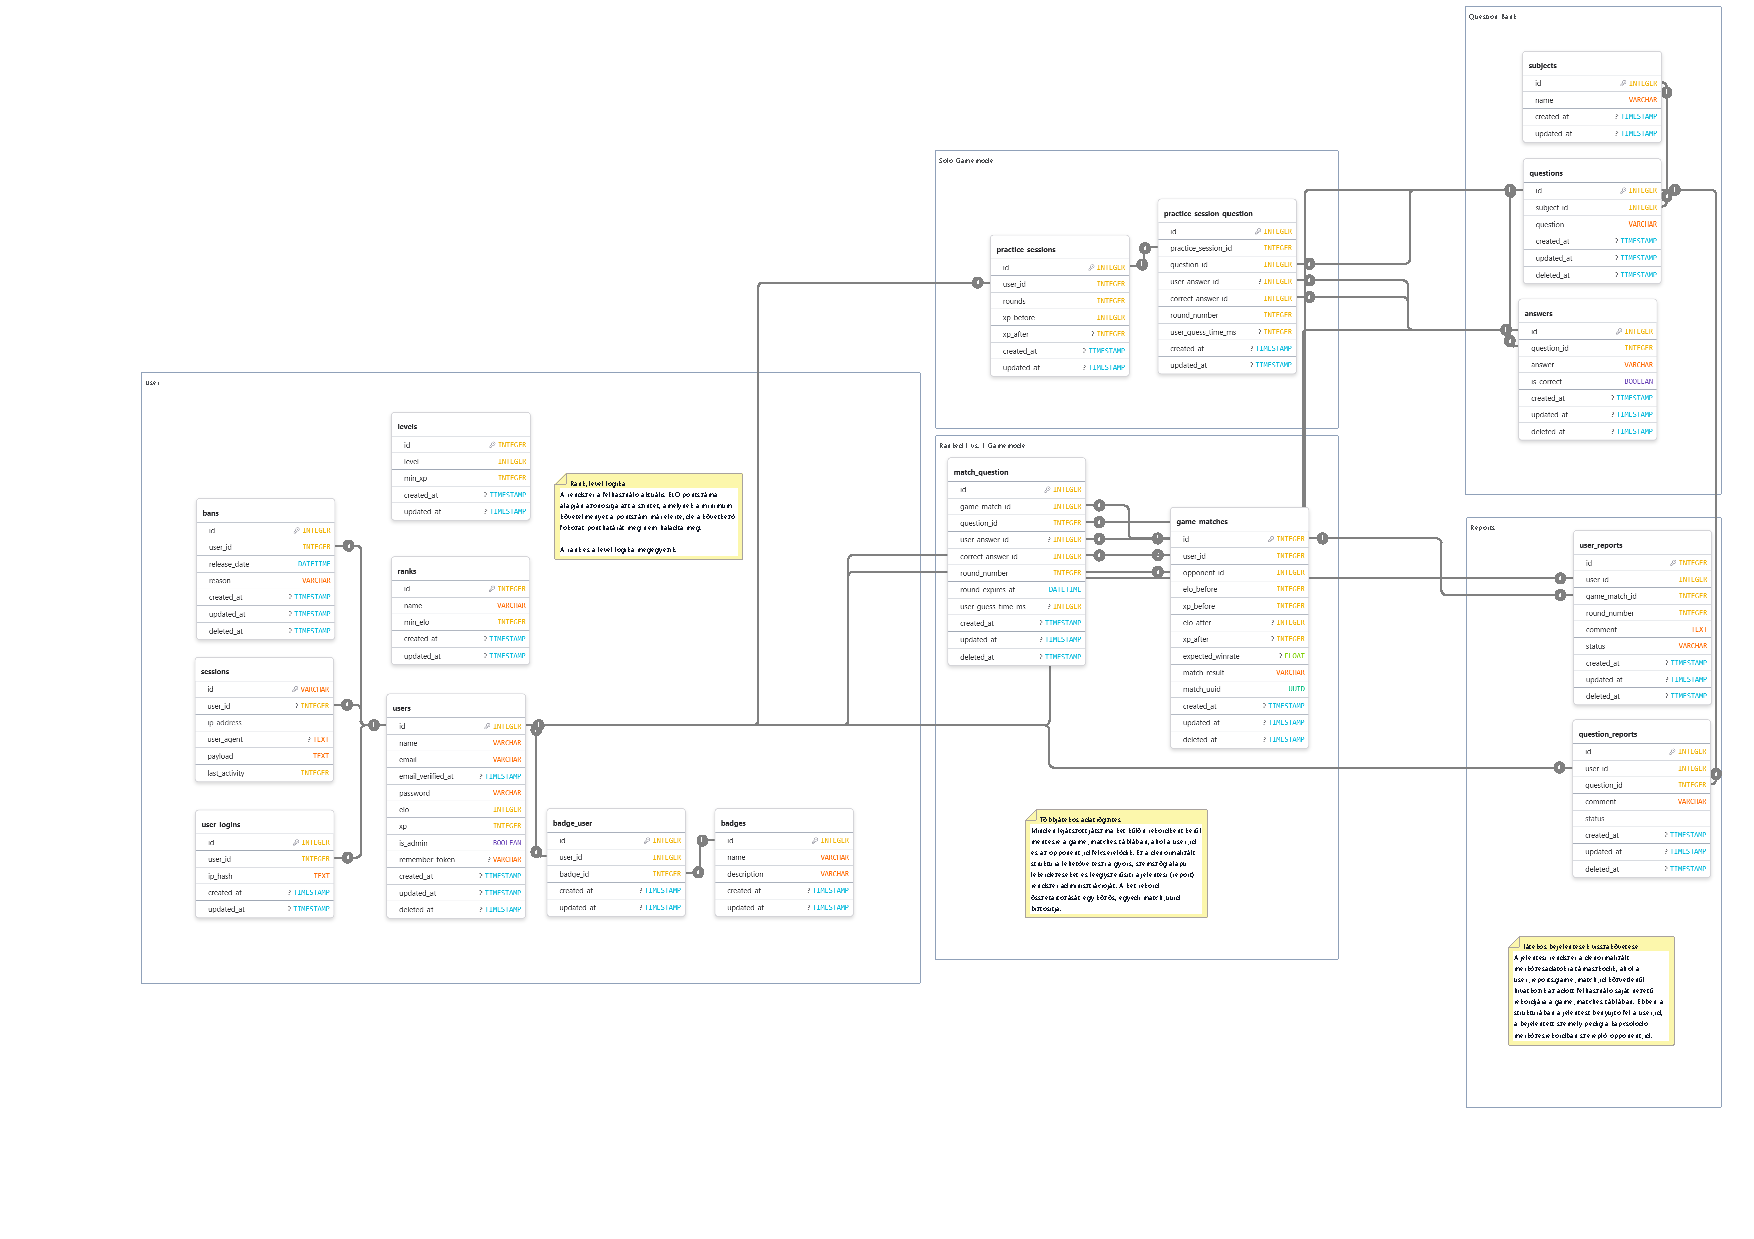
\includegraphics[width=\textwidth]{images/er-diagram.pdf} 
    \caption{A SkillIssue alkalmazás ER diagramja}
    \label{fig:er_diagram}
\end{figure}

\subsection{Entitások leírása}
A rendszer főbb entitásai és azok szerepkörei:

\begin{itemize}
    \item \textbf{users:} A felhasználók alapvető adatait, kompetitív rangját (ELO), tapasztalati pontjait (XP) és adminisztrátori jogosultságait tárolja.
    \item \textbf{questions \& answers:} A kvízjáték magját alkotó kérdések és a hozzájuk tartozó helyes/helytelen válaszlehetőségek tárolóhelye, tantárgyak (subjects) szerint csoportosítva.
    \item \textbf{game\_matches:} A felhasználók közötti párbajok adatait rögzíti. A gyors lekérdezhetőség és az adatbázis kapcsolatok egyszerűsítésének érdekében redundáns (denormalizált) módon tárolja a meccseket, minden résztvevő szemszögéből egy-egy rekorddal.
    \item \textbf{match\_question:} A mérkőzések során feltett konkrét kérdéseket, a felhasználó válaszait és a válaszidőket rögzíti körökre bontva.
    \item \textbf{practice\_sessions:} A gyakorló mód adatait tárolja, ahol a felhasználó tét nélkül (ELO változás nélkül) szerezhet tapasztalatot.
    \item \textbf{reports:} Felhasználó és kérdés jelentések kezelésére szolgáló entitások a platform moderációjához.
    \item \textbf{bans \& logins:} Biztonsági entitások, amelyek a kitiltások és a bejelentkezési előzmények (IP hash) nyomon követésére szolgálnak.
\end{itemize}

\subsection{Kapcsolatok és megszorítások}
Az adatbázis integritását az alábbi főbb kapcsolatok és megszorítások biztosítják:

\begin{enumerate}
    \item \textbf{Egy-a-többhöz (1:N) kapcsolatok:}
    \begin{itemize}
        \item Egy \texttt{subject} több \texttt{question}-höz kapcsolódik.
        \item Egy \texttt{question}-höz több \texttt{answer} tartozik.
        \item Egy \texttt{user} több mérkőzéssel (\texttt{game\_matches}), gyakorlással (\texttt{practice\_sessions}) és jelentéssel rendelkezhet.
    \end{itemize}
    
    \item \textbf{Több-a-többhöz (N:M) kapcsolatok:}
    \begin{itemize}
        \item A felhasználók és badge-ek kapcsolata a \texttt{badge\_user} kapcsolótáblán keresztül valósul meg.
    \end{itemize}

    \item \textbf{Egyediségi megszorítások (Unique):}
    Az e-mail címek, a rangok minimum pontszámai (\texttt{min\_elo}) és a szintek (\texttt{min\_xp}) egyedisége biztosítja, hogy a rangsorolási és azonosítási rendszer egyértelmű maradjon.
    
    \item \textbf{Denormalizációs stratégia:}
    A \texttt{game\_matches} tábla szándékosan duplikált rekordokat tárol (minden meccset kétszer, felcserélt \texttt{user\_id} és \texttt{opponent\_id} mezőkkel), amit egy közös \texttt{match\_uuid} fog össze. Ez egyszerűsíti a lekérdezési folyamatot több adatbázis kapcsolaton keresztül.
\end{enumerate}